\subsection{Umfrage erstellen}
\label{ssec:konzept:client:umfrage_erstellen}

Die eigentliche Aufgabe der Anwendung neben der Auswertung von Umfragen ist es, diese zuvor zu erstellen bzw. zu konzipieren.
Hierfür soll die Anwendung die Möglichekeit bieten Fragen der Art \emph{Single Choice}, \emph{Multiple Choice}, \emph{Rating} und \emph{offene Fragen} zu erstellen.
Mock-Ups, welche die Erstellung der einzelnen Fragekategorien zeigen, sind in den Abbildungen \ref{MockUmfrageSingleChoice}, \ref{MockUmfrageOffeneFragen} sowie in den Abbbildungen im Anhang \ref{MockUmfrageMultipleChoice}, \ref{MockUmfrageRating} zu sehen.
Die Art der Frage kann dabei über ein Dropdown-Feld bestimmt werden.
Bei jeder Frage soll ein Textfeld mit der eigentlichen Frage angeboten werden.
Im Fall von Single- und Multiple-Choice-Fragen soll die Möglichkeit bestehen weitere Antwortmöglichkeiten hinzuzufügen.
Bei Rating- bzw. skalierten Fragen soll es eine Möglichkeit geben die Skalierung anpassen zu können.
Hierzu sind die in  Abbildung  \ref{MockUmfrageRating} zu sehende \emph{von} bzw. \emph{bis} Feld genutzt werden.


% Das Herzstück der Applikation soll das Erstellen einer Umfrage sein. 
% Hier soll der Benutzer die Möglichkeit haben, eine Umfrage zu erstellen, die verschiedene Fragetypen beinhaltet. 
% Der Benutzer soll einen Titel sowie eine Beschreibung seiner Umfrage definieren können. 
% Darüber hinaus soll diese erstellte Umfrage als Vorlage \emph{(engl. Template)} dienen, um basierend auf ihr verschiedene Umfragen erstellen zu können oder auch eine bestehende Umfrage erweitern zu können. 
% Diese soll dann über einen neuen \emph{Sourveycode} realisiert werden. 

% Abb. \myRefGeneral{fig:MockUmfrageErstellen} stellt ein Mockup dar, indem der Benutzer seine Umfragen einsehen kann. 
% Die Umfragen sollen spezifisch nur für den angemeldeten Benutzer sichbar sein. 
% Zudem soll der Benutzer noch die Möglichkeit haben, über eine Suchfunktion in seinen Umfragen nach einer geeigneten Umfrage zu suchen. \newline
% Darüberhinaus soll dem Benutzer visuell dargestellt werden, wieviele Umfragen er basierend auf dieser Vorlage (Master Survey) erstellt hat. 
% Des weiteren soll dem Benutzer ermöglicht werden, Umfragen, die noch nicht veröffentlich wurden, zu editieren und zu löschen. \newline
% Über eine Button \enquote{Publish survey} soll der Benutzer eine Umfrage basierend auf dieser Master Survey erstellen können. 
% Ihm soll visuell dargestellt werden, dass das Anlegen erfolgreich war und den generierten Sourveycode anzeigen. 
% Diese wird seinem Result-Dashboard hinzugefügt (Kap. \myRefGeneral{ssec:ResultDashboard}). 

\begin{figure}[h]
	\centering
	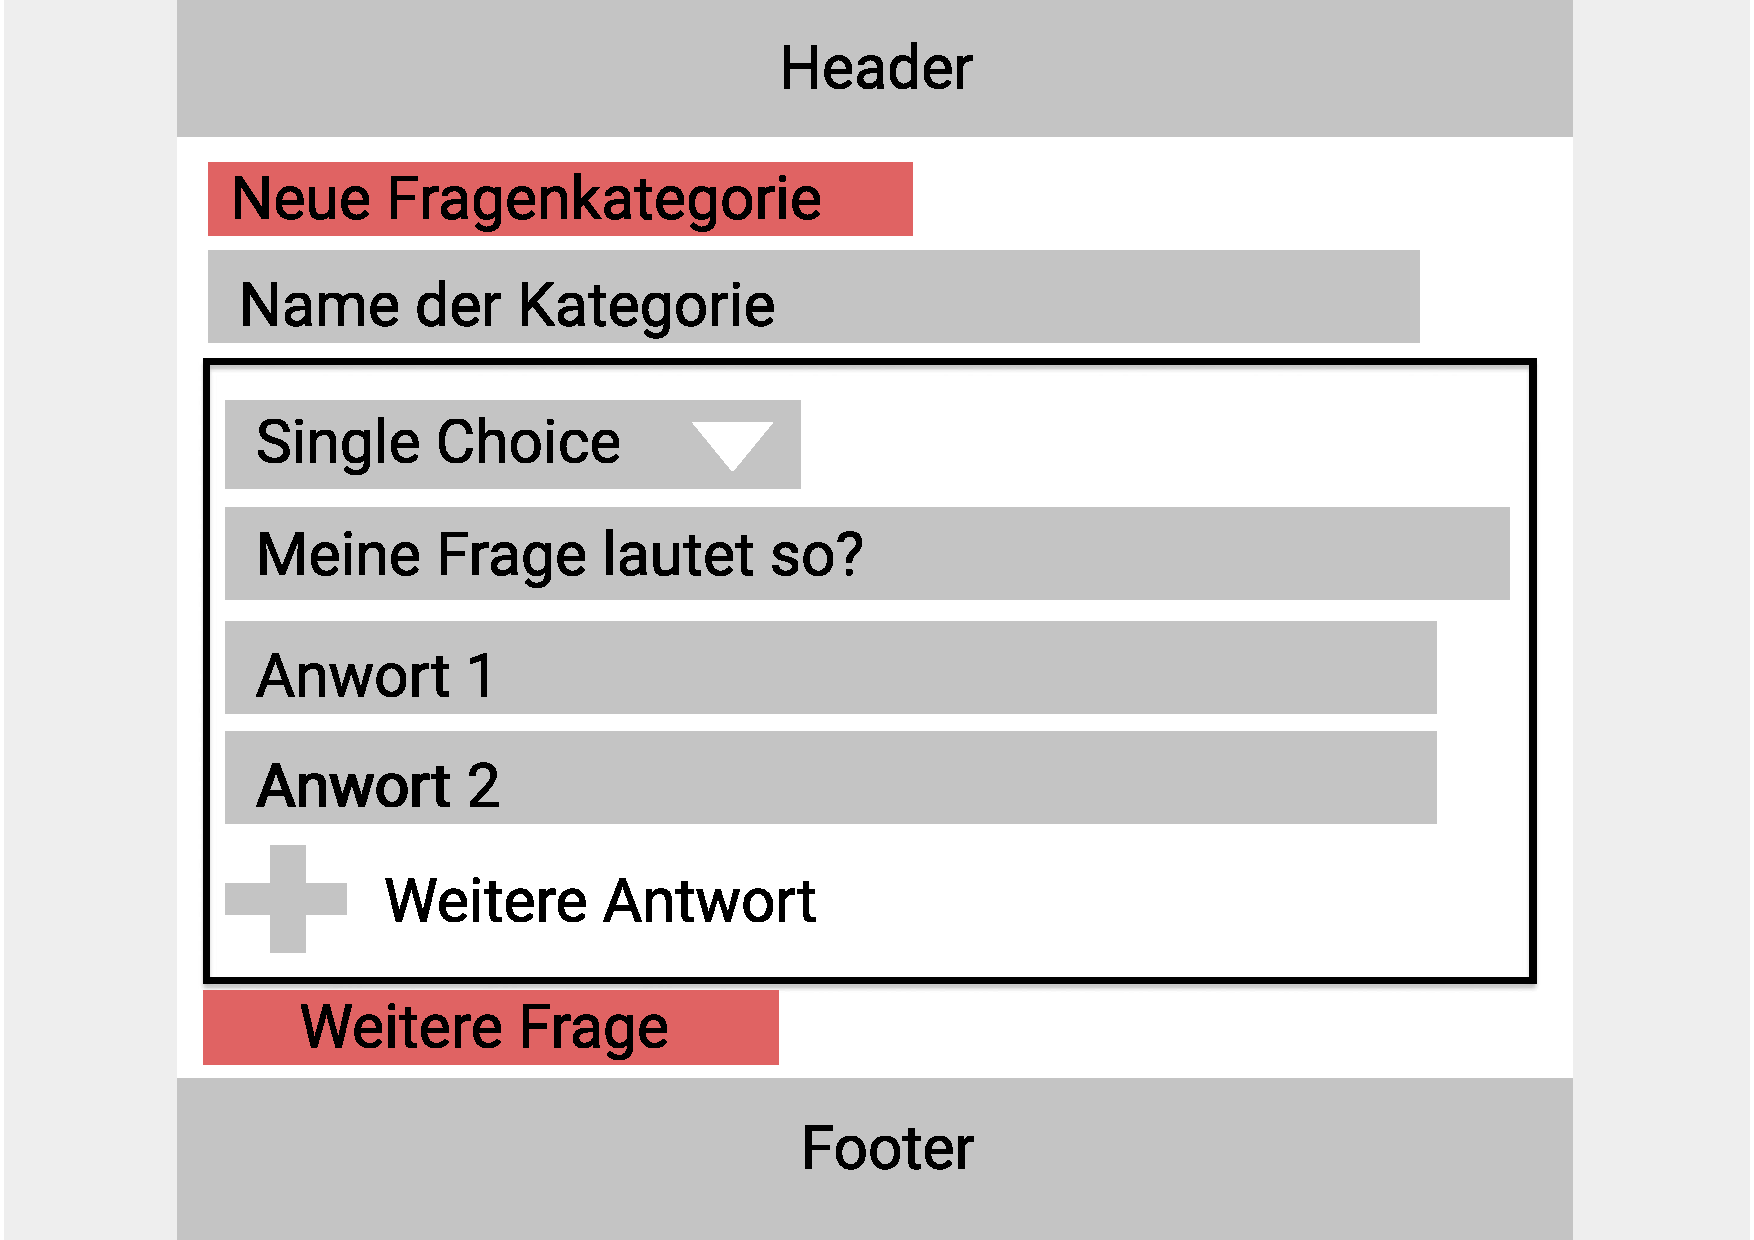
\includegraphics[width=0.7\textwidth]{img/konzeption/client/umfrage_erstellen_single_choice}
	\captionsetup{justification=centering, format=plain}
	\caption[Mock-Up der Umfrageerstellung von Single-Choice-Fragen]{Mock-Up der Umfrageerstellung von Single-Choice-Fragen\\\figma}
	\label{fig:MockUmfrageSingleChoice}
\end{figure}

\begin{figure}[h]
	\centering
	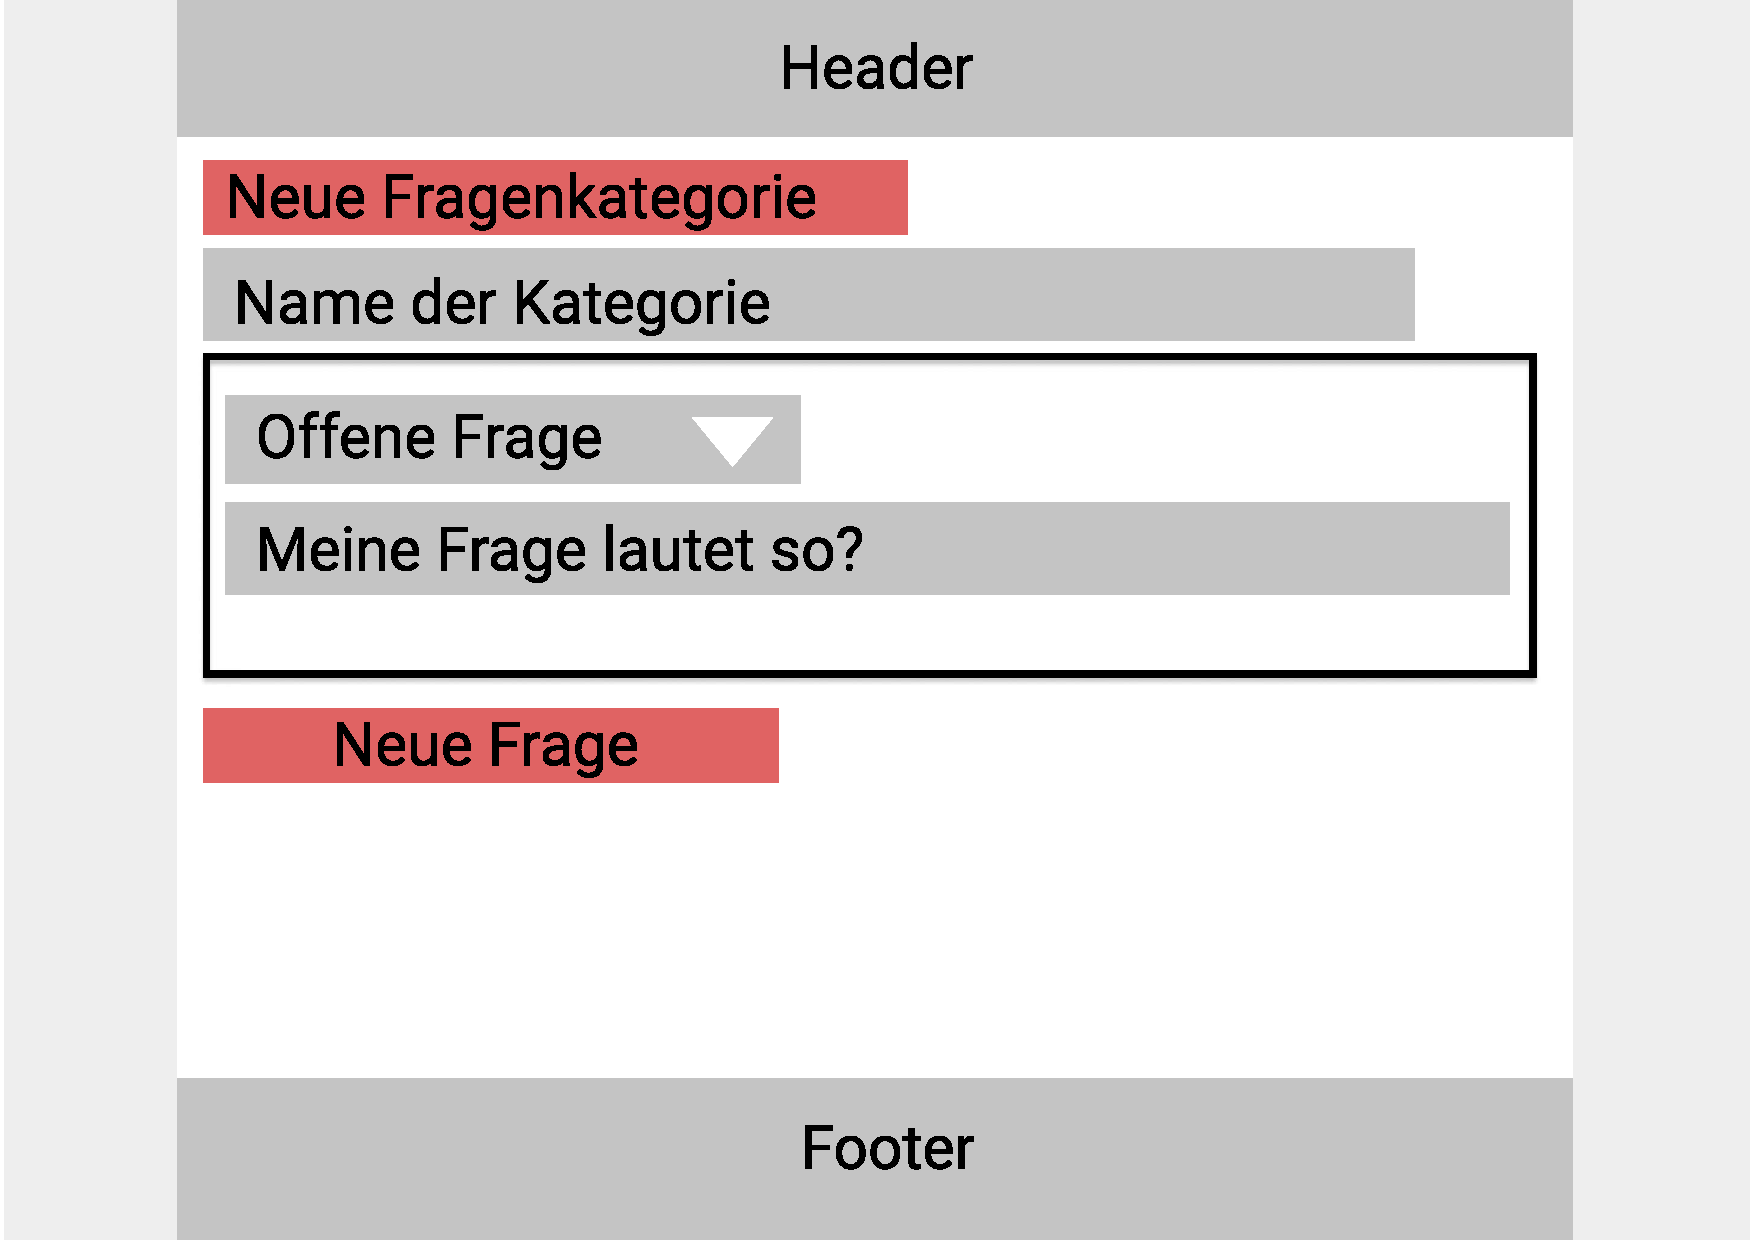
\includegraphics[width=0.7\textwidth]{img/konzeption/client/umfrage_erstellen_offene_frage}
	\captionsetup{justification=centering, format=plain}
	\caption[Mock-Up der Umfrageerstellung von offenen Fragen]{Mock-Up der Umfrageerstellung von offenen Fragen\\\figma}
	\label{fig:MockUmfrageOffeneFragen}
\end{figure}
